\documentclass[10pt, letterpaper]{article}

%% Packages %%
\usepackage[left=2cm,top=3cm,right=2cm,bottom=2cm]{geometry}
\usepackage{graphicx}
\usepackage[spanish]{babel}
\usepackage[latin1]{inputenc}
\usepackage{amsmath, amsfonts, amssymb, amsthm}
\usepackage{array, xcolor}
\usepackage{chngcntr}
\usepackage{booktabs}
\usepackage{enumitem}
\usepackage{multirow}
\usepackage[font=footnotesize]{caption}

%% Document format %%
%\pagestyle{myheadings}       % Uncomment if don't want page numbers
%\markright{MUC863 Psicoac�stica}
\linespread{1.0}
\setlength{\parindent}{0pt}
\setlist{noitemsep}
\setlist{nolistsep}

%% Comandos %%
\definecolor{lightgray}{gray}{0.8}
\newcommand{\newsection}[1]{\setcounter{section}{#1} \setcounter{figure}{0} \setcounter{table}{0} \setcounter{equation}{0}}
\newcommand\VRule{\color{lightgray}\vrule width 0.5pt}
\newcommand{\extend}[2]{#1 \hfill #2}
\newcommand{\extendbf}[2]{\textbf{#1 \hfill #2}}

%% Otros %%
\counterwithin{equation}{section}
\counterwithin{figure}{section}
\counterwithin{table}{section}

\title{Tarea 3 - An�lisis de formantes}
\author{Nicol�s A. Pe�a Escarpentier}
\date{} 

\begin{document}
\maketitle

\section*{Pregunta 1} \newsection{1}

Mediante el programa ``Praat'' grab� las cinco vocales para posteriormente analizar sus formantes y sus trayectorias. Las tres primeras formantes pueden ser vistas en la tabla \ref{1tab_formantes}  y los gr�ficos de las trayectorias de las formantes en la figura \ref{1fig_formantes}.

\begin{table}[htbp]
  \centering
    \begin{tabular}{cccccc}
    \toprule
          & \multicolumn{5}{c}{Vocal} \\
          & a     & e     & i     & o     & u \\
    \midrule
    {F1} &  447.9 & 1073.0 &  245.2 &  815.9 &  239.8 \\
    {F2} & 1134.4 & 2284.5 & 2181.8 & 2255.9 &  786.4 \\
    {F3} & 2602.3 & 3140.5 & 3095.0 & 3153.0 & 2305.1 \\
    \bottomrule
    \end{tabular}%
  \caption{Formantes de las cinco vocales}
  \label{1tab_formantes}%
\end{table}%

\begin{figure}[h!]
\centering
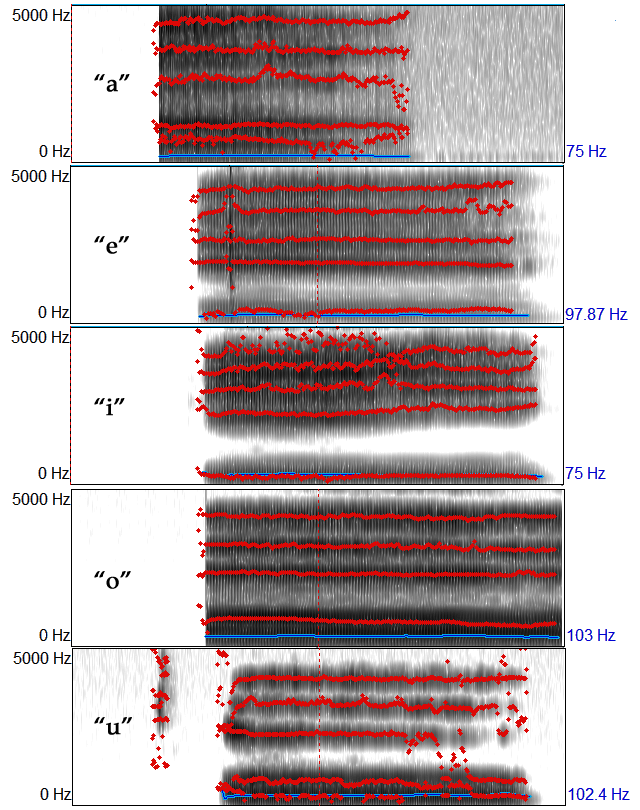
\includegraphics[scale=0.6]{formantes.png}
\caption{Trayectoria de las formantes}
\label{1fig_formantes}
\end{figure}

Es posible apreciar que la frecuencia de las formantes se mantiene bastante uniforme a lo largo de su trayectoria. Para la vocal ``u'' se puede apreciar un ruido inicial, el cual es producto de error m�o a la hora de grabar. Adem�s, las l�neas hechas por el programa tienen ciertos errores debido a una grabaci�n muy baja que hice de esa vocal. Por otra parte, es posible ver claramente que frecuencias corresponden a cada vocal y que dichas frecuencias no afectan al pitch de mi voz (n�mero al extremo derecho de cada espectrograma.

\newpage \quad \newpage
\section*{Pregunta 2} \newsection{2}
Se escogi� una consonante de cada grupo y se junt� con cada una de las vocales, con el fin de analizar y graficar las formantes. Para cada caso, analizaremos la consonante junto a la vocal ``a'', puesto que el an�lisis del resto de las vocales es similar. \\

\begin{itemize}
\item \textbf{Plosiva}: ``t''\\
En este caso, podemos apresiar un ruido inicial, bastante breve, que eleva la frecuencia de las formantes, para luego bajar a formar la vocal correspondiente. \\

\item \textbf{Fricativa}: ``f''\\
En este caso, se puede observar que al pronunciar la consonante, se produce un sonido levemente ruidoso, de mayor frecuencia y larga duraci�n, el que luego baja hacia la frecuencia de la formante respectiva.\\

\item \textbf{Nasal}: ``n''\\
En este caso, el ruido inicial altera las formantes de distintas maneras. La primera formante baja mucho su frecuencia, la segunda la sube y la tercera la sube en menor medida. Luego, al pronunciar la vocal, las formantes se tienden a normalizar a las frecuencias que corresponden a la vocal.\\

\item \textbf{Semivocal}: ``y''\\
En este caso, es posible apreciar que el sonido es equivalente a pronunciar primero una ``i'' que luego pasa a otra vocal, pero con un peque��simo ruido al comienzo.\\

\item \textbf{L�quida}: ``l''\\
En este caso, se puede observar claramente una estructura de formantes inicial, correspondiente a la consonante, que luego da paso a la vocal respectiva.
\end{itemize}
\bigskip

Se puede ver la trayectoria de las formantes en la tabla \ref{2tab_consonantes} y en la figura \ref{2fig_formantes}. Los tiempos $t_1$, $t_2$ y $t_3$ fueron tomados arbitrariamente, con tal de mostrar efectivamente algunos valores de la trayectoria de las formantes. Mirando los valores de la tabla, es posible darse cuenta que partiendo del ruido inicial, se forma la trayectoria necesaria para terminar formando la vocal correspondiente. Si nos fijamos en los valores finales, estos siempre son bastante similares, correspondientes a la vocal que se est� pronunciando.

\begin{table}[htbp]
  \centering
    \begin{tabular}{rrccc}
    \toprule
    & & \multicolumn{3}{c}{Tiempo} \\
    \multicolumn{1}{c}{} & \multicolumn{1}{c}{} & $t_1$ & $t_2$ & $t_3$ \\
    \midrule
    \multicolumn{1}{c}{\multirow{3}[2]{*}{``ta''}} &  F1   & 761.6 & 1370.3 & 642.9 \\
    \multicolumn{1}{c}{} &  F2   & 1713.1 & 1785.3 & 1458.5 \\
    \multicolumn{1}{c}{} &  F3   & 2840.3 & 2837.5 & 2600.6 \\
    \midrule
    \multicolumn{1}{c}{\multirow{3}[2]{*}{``fa''}} &  F1   & 2064.9 & 1457.0 & 636.7 \\
    \multicolumn{1}{c}{} &  F2   & 2441.0 & 2083.4 & 1273.6 \\
    \multicolumn{1}{c}{} &  F3   & 3677.9 & 3171.4 & 2299.0 \\
    \midrule
    \multicolumn{1}{c}{\multirow{3}[2]{*}{``na''}} &  F1   & 228.9 & 364.6 & 595.5 \\
    \multicolumn{1}{c}{} &  F2   & 2026.3 & 1430.1 & 1658.1 \\
    \multicolumn{1}{c}{} &  F3   & 2511.5 & 2525.5 & 2026.2 \\
    \midrule
    \multicolumn{1}{c}{\multirow{3}[2]{*}{``ya''}} &  F1   & 245.4 & 405.6 & 654.9 \\
    \multicolumn{1}{c}{} &  F2   & 2073.6 & 1989.4 & 1558.1 \\
    \multicolumn{1}{c}{} &  F3   & 3001.1 & 2649.4 & 2241.0 \\
    \midrule
    \multicolumn{1}{c}{\multirow{3}[2]{*}{``la''}} &  F1   & 200.3 & 329.0 & 634.2 \\
    \multicolumn{1}{c}{} &  F2   & 1579.9 & 1627.9 & 1603.8 \\
    \multicolumn{1}{c}{} &  F3   & 2368.4 & 3026.9 & 2485.3 \\
    \bottomrule
    \end{tabular}%
  \caption{Trayectoria de formantes de consonante + vocal}
  \label{2tab_consonantes}%
\end{table}%

\begin{figure}[h!]
\centering
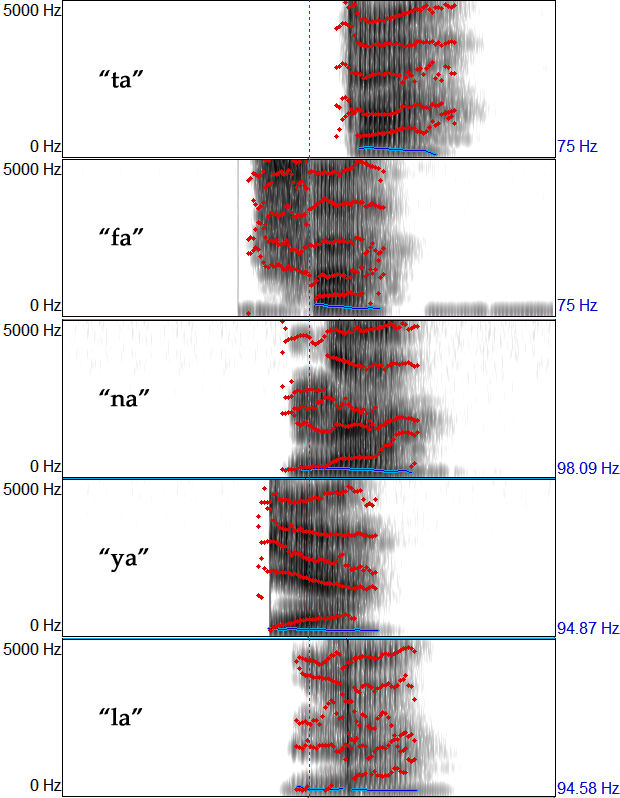
\includegraphics[scale=0.6]{cons_formantes.png}
\caption{Trayectoria de las formantes de consonantes con vocales}
\label{2fig_formantes}
\end{figure}


\end{document}